\documentclass[a4paper,10pt]{article}

%%%%%%%%%%%%%%%%%%%%%%%%%%%%%%%%%%%%%%%%

\usepackage{graphicx}
\usepackage[english]{babel}
\usepackage[latin1]{inputenc}
\usepackage{pgfplots}

\pgfplotsset{width=10cm,compat=1.9}

%%%%%%%%%%%%%%%%%%%%%%%%%%%%%%%%%%%%%%%%

\begin{document}

%%%%%%%%%%%%%%%%%%%%%%%%%%%%%%%%%%%%%%%%
% Frontpage

\title{Parallelizing Haskell Program Coverage code\\
  \Large{A story of tears and fear}
}
\author{Agust\'in Mista\\ mista@chalmers.se}
\date{}
\maketitle

%%%%%%%%%%%%%%%%%%%%%%%%%%%%%%%%%%%%%%%%
% Sections

\section*{Introduction}

Pellentesque dapibus suscipit ligula. Donec posuere augue in quam. Etiam vel
tortor sodales tellus ultricies commodo. Suspendisse potenti. Aenean in sem ac
leo mollis blandit. Donec neque quam, dignissim in, mollis nec, sagittis eu,
wisi. Phasellus lacus. Etiam laoreet quam sed arcu. Phasellus at dui in ligula
mollis ultricies. Integer placerat tristique nisl. Praesent augue. Fusce
commodo. Vestibulum convallis, lorem a tempus semper, dui dui euismod elit,
vitae placerat urna tortor vitae lacus. Nullam libero mauris, consequat quis,
varius et, dictum id, arcu. Mauris mollis tincidunt felis. Aliquam feugiat
tellus ut neque. Nulla facilisis, risus a rhoncus fermentum, tellus tellus
lacinia purus, et dictum nunc justo sit amet elit.

\subsection*{Sequential implementations}

% Sequential times
\resizebox{\textwidth}{!}{
\hspace{-50pt}
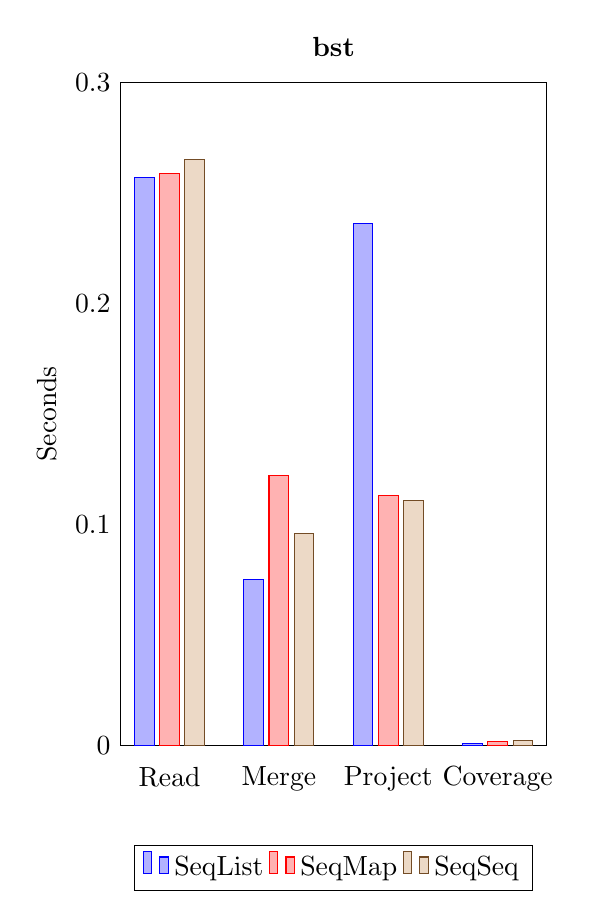
\begin{tikzpicture}
  \pgfplotsset{xtick style={draw=none}}
  \pgfplotsset{ytick style={draw=none}}
  \begin{axis}[
      bar width=0.25cm,
      width=7cm,
      height=10cm,
      ybar,
      enlargelimits=0.15,
      legend style={
        at={(0.5,-0.15)},
        anchor=north,legend columns=-1
      },
      enlarge y limits=0,
      ymax=0.3,
      ymin=0,
      ytick distance=0.1,
      xtick=data,
      title={\textbf{bst}},
      ylabel={Seconds},
      symbolic x coords={Read, Merge, Project, Coverage},
    ]
    \addplot coordinates {(Read,0.257) (Merge,0.075) (Project,0.236) (Coverage, 0.0007)};
    \addplot coordinates {(Read,0.259) (Merge,0.122) (Project,0.113) (Coverage, 0.0018)};
    \addplot coordinates {(Read,0.265) (Merge,0.096) (Project,0.111) (Coverage, 0.0020)};
    \legend{SeqList, SeqMap, SeqSeq}
  \end{axis}
\end{tikzpicture}
~\hspace{-15pt}
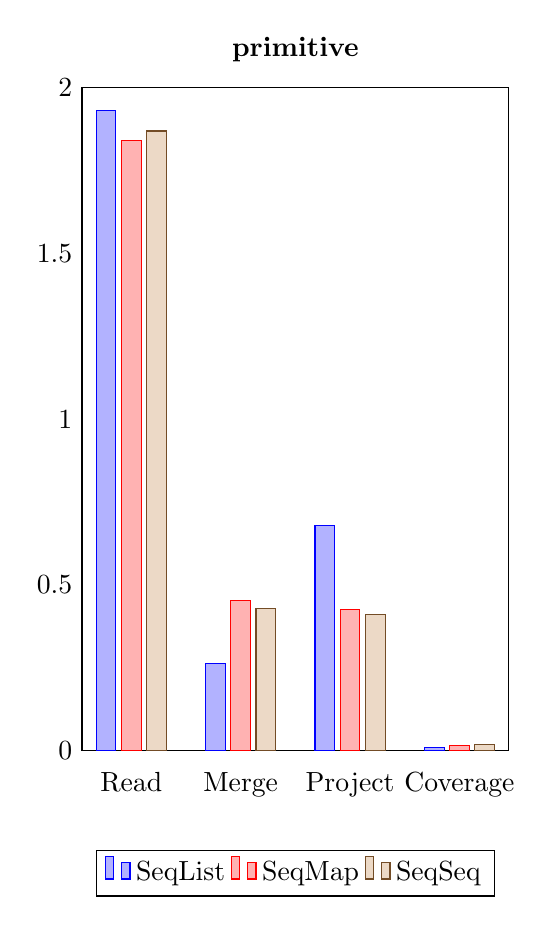
\begin{tikzpicture}
  \pgfplotsset{xtick style={draw=none}}
  \pgfplotsset{ytick style={draw=none}}
  \begin{axis}[
      bar width=0.25cm,
      width=7cm,
      height=10cm,
      ybar,
      enlargelimits=0.15,
      legend style={
        at={(0.5,-0.15)},
        anchor=north,legend columns=-1
      },
      enlarge y limits=0,
      ymax=2,
      ymin=0,
      ytick distance=0.5,
      xtick=data,
      title={\textbf{primitive}},
      symbolic x coords={Read, Merge, Project, Coverage},
    ]
    \addplot coordinates {(Read,1.931) (Merge,0.262) (Project,0.680) (Coverage, 0.010)};
    \addplot coordinates {(Read,1.841) (Merge,0.452) (Project,0.426) (Coverage, 0.015)};
    \addplot coordinates {(Read,1.870) (Merge,0.429) (Project,0.412) (Coverage, 0.018)};
    \legend{SeqList, SeqMap, SeqSeq}
  \end{axis}
\end{tikzpicture}
~\hspace{-15pt}
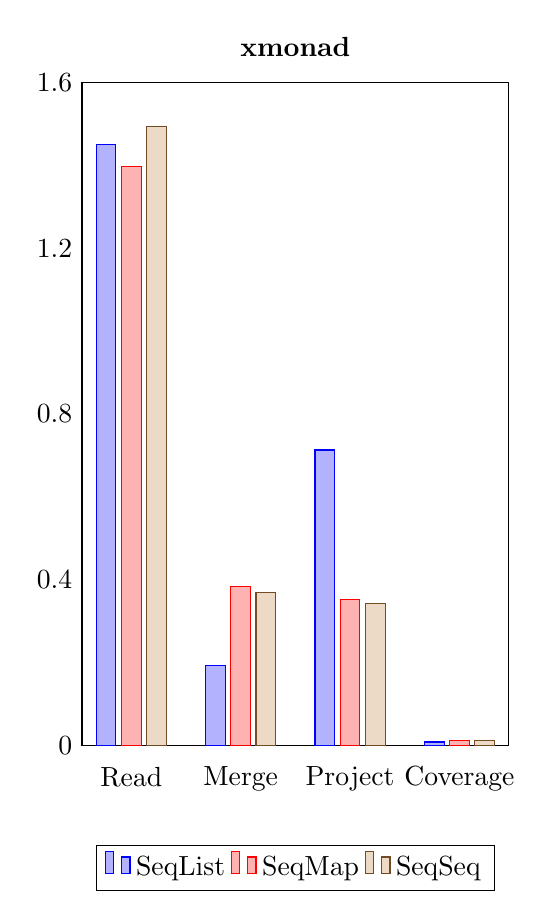
\begin{tikzpicture}
  \pgfplotsset{xtick style={draw=none}}
  \pgfplotsset{ytick style={draw=none}}
  \begin{axis}[
      bar width=0.25cm,
      width=7cm,
      height=10cm,
      ybar,
      enlargelimits=0.15,
      legend style={
        at={(0.5,-0.15)},
        anchor=north,legend columns=-1
      },
      enlarge y limits=0,
      ymax=1.6,
      ymin=0,
      ytick distance=0.4,
      xtick=data,
      title={\textbf{xmonad}},
      symbolic x coords={Read, Merge, Project, Coverage},
    ]
    \addplot coordinates {(Read,1.450) (Merge,0.193) (Project,0.713) (Coverage, 0.008)};
    \addplot coordinates {(Read,1.398) (Merge,0.383) (Project,0.353) (Coverage, 0.011)};
    \addplot coordinates {(Read,1.493) (Merge,0.368) (Project,0.343) (Coverage, 0.012)};
    \legend{SeqList, SeqMap, SeqSeq}
  \end{axis}
\end{tikzpicture}
}

% Zoomed coverage
\resizebox{0.4\textwidth}{!}{
\hspace{-50pt}
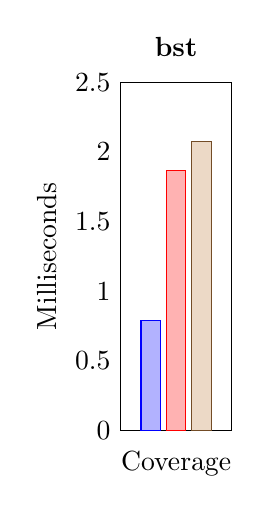
\begin{tikzpicture}
  \pgfplotsset{xtick style={draw=none}}
  \pgfplotsset{ytick style={draw=none}}
  \begin{axis}[
      bar width=0.25cm,
      width=3cm,
      height=6cm,
      ybar,
      enlargelimits=0.15,
      enlarge y limits=0,
      ymax=2.5,
      ymin=0,
      ytick distance=0.5,
      xtick=data,
      ylabel={Milliseconds},
      title={\textbf{bst}},
      symbolic x coords={Read, Merge, Project, Coverage},
    ]
    \addplot coordinates {(Coverage, 0.791)};
    \addplot coordinates {(Coverage, 1.870)};
    \addplot coordinates {(Coverage, 2.076)};
    \legend{}
  \end{axis}
\end{tikzpicture}
~\hspace{-5pt}
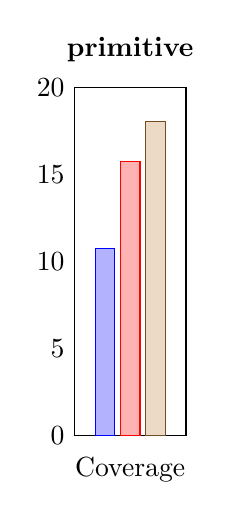
\begin{tikzpicture}
  \pgfplotsset{xtick style={draw=none}}
  \pgfplotsset{ytick style={draw=none}}
  \begin{axis}[
      bar width=0.25cm,
      width=3cm,
      height=6cm,
      ybar,
      enlargelimits=0.15,
      enlarge y limits=0,
      ymax=20,
      ymin=0,
      ytick distance=5,
      xtick=data,
      title={\textbf{primitive}},
      symbolic x coords={Read, Merge, Project, Coverage},
    ]
    \addplot coordinates {(Coverage, 10.78)};
    \addplot coordinates {(Coverage, 15.77)};
    \addplot coordinates {(Coverage, 18.09)};
    \legend{}
  \end{axis}
\end{tikzpicture}
~\hspace{-5pt}
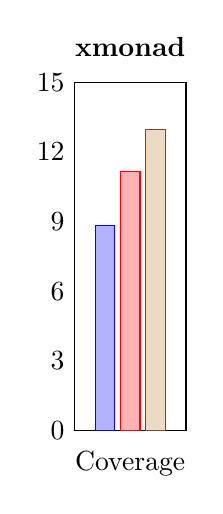
\begin{tikzpicture}
  \pgfplotsset{xtick style={draw=none}}
  \pgfplotsset{ytick style={draw=none}}
  \begin{axis}[
      bar width=0.25cm,
      width=3cm,
      height=6cm,
      ybar,
      enlargelimits=0.15,
      enlarge y limits=0,
      ymax=15,
      ymin=0,
      ytick distance=3,
      xtick=data,
      title={\textbf{xmonad}},
      symbolic x coords={Read, Merge, Project, Coverage},
    ]
    \addplot coordinates {(Coverage, 8.843)};
    \addplot coordinates {(Coverage, 11.150)};
    \addplot coordinates {(Coverage, 12.986)};
    \legend{}
  \end{axis}
\end{tikzpicture}
}

\subsection*{Parallel Read}

\includegraphics[scale=0.3]{threadscope/ParRead}

% Parallel read
\resizebox{\textwidth}{!}{
\hspace{-50pt}
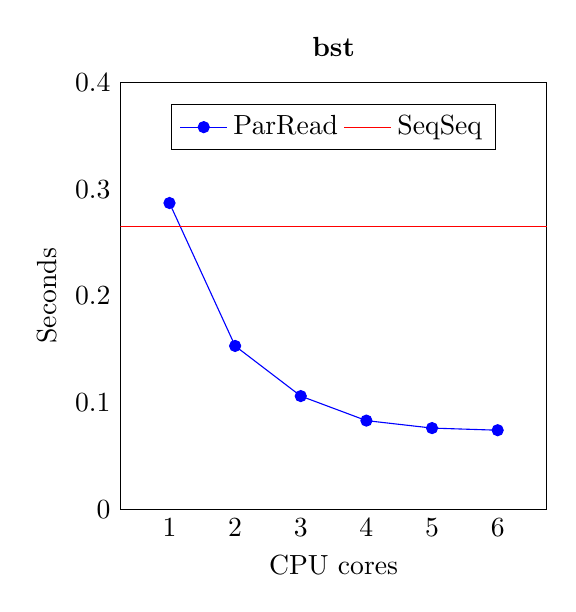
\begin{tikzpicture}
  \pgfplotsset{xtick style={draw=none}}
  \pgfplotsset{ytick style={draw=none}}
  \begin{axis}[
      width=7cm,
      height=7cm,
      enlargelimits=0.15,
      enlarge y limits=0,
      ymax=0.4,
      ymin=0,
      ytick distance=0.1,
      xtick=data,
      ylabel={Seconds},
      xlabel={CPU cores},
      xmin=1,
      xmax=6,
      xtick distance=1,
      title={\textbf{bst}},
      legend style={
        at={(0.5,0.95)},
        anchor=north,legend columns=-1
      }
    ]
    \addplot[mark=*, blue] coordinates {
      (1, 0.287)
      (2, 0.153)
      (3, 0.106)
      (4, 0.083)
      (5, 0.076)
      (6, 0.074)
    };
    \addplot[mark=none, red] coordinates {
      (0,0.265) (7,0.265)
    };
    \legend{ParRead, SeqSeq}
  \end{axis}
\end{tikzpicture}
~\hspace{-5pt}
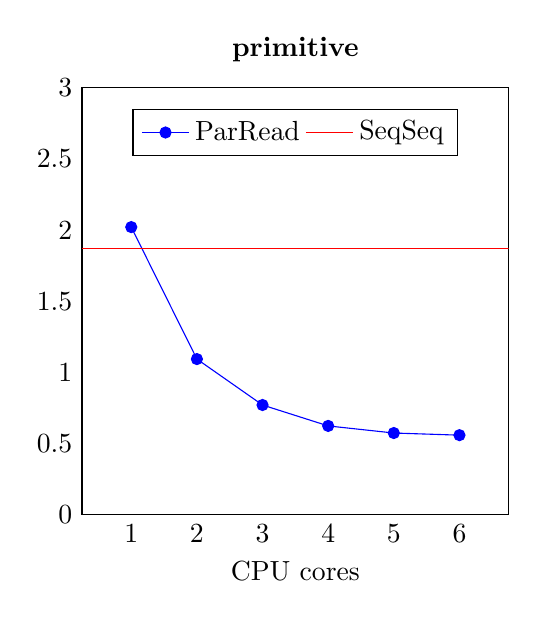
\begin{tikzpicture}
  \pgfplotsset{xtick style={draw=none}}
  \pgfplotsset{ytick style={draw=none}}
  \begin{axis}[
      width=7cm,
      height=7cm,
      enlargelimits=0.15,
      enlarge y limits=0,
      ymax=3,
      ymin=0,
      ytick distance=0.5,
      xtick=data,
      xlabel={CPU cores},
      xmin=1,
      xmax=6,
      xtick distance=1,
      title={\textbf{primitive}},
      legend style={
        at={(0.5,0.95)},
        anchor=north,legend columns=-1
      }
    ]
    \addplot[mark=*, blue] coordinates {
      (1, 2.021)
      (2, 1.093)
      (3, 0.770)
      (4, 0.623)
      (5, 0.573)
      (6, 0.558)
    };
    \addplot[mark=none, red] coordinates {
      (0,1.870) (7,1.870)
    };
    \legend{ParRead, SeqSeq}
  \end{axis}
\end{tikzpicture}
~\hspace{-5pt}
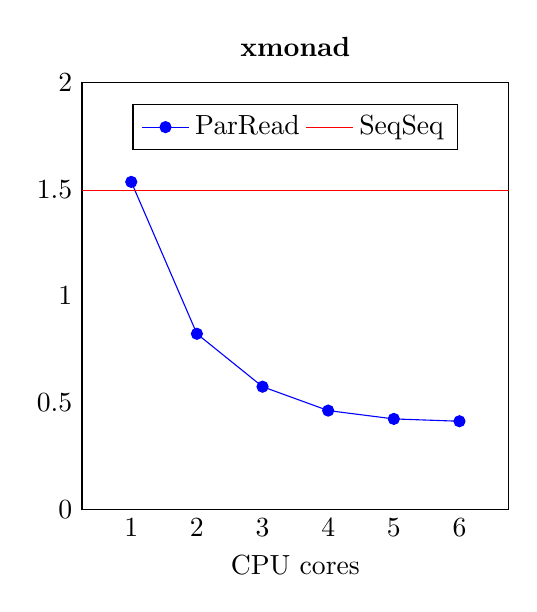
\begin{tikzpicture}
  \pgfplotsset{xtick style={draw=none}}
  \pgfplotsset{ytick style={draw=none}}
  \begin{axis}[
      width=7cm,
      height=7cm,
      enlargelimits=0.15,
      enlarge y limits=0,
      ymax=2,
      ymin=0,
      ytick distance=0.5,
      xtick=data,
      xlabel={CPU cores},
      xmin=1,
      xmax=6,
      xtick distance=1,
      title={\textbf{xmonad}},
      legend style={
        at={(0.5,0.95)},
        anchor=north,legend columns=-1
      }
    ]
    \addplot[mark=*, blue] coordinates {
      (1, 1.534)
      (2, 0.822)
      (3, 0.574)
      (4, 0.462)
      (5, 0.423)
      (6, 0.412)
    };
    \addplot[mark=none, red] coordinates {
      (0,1.493) (7,1.493)
    };
    \legend{ParRead, SeqSeq}
  \end{axis}
\end{tikzpicture}
}

\subsection*{Parallel Merge}

\includegraphics[scale=0.3]{threadscope/ParMerge1}

\includegraphics[scale=0.3]{threadscope/ParMerge2}

\includegraphics[scale=0.3]{threadscope/ParMerge3}


% Parallel merge
\resizebox{\textwidth}{!}{
\hspace{-50pt}
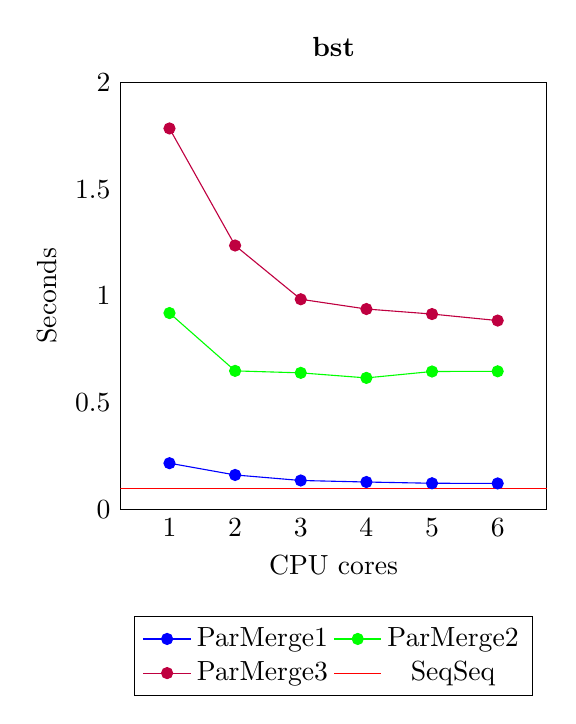
\begin{tikzpicture}
  \pgfplotsset{xtick style={draw=none}}
  \pgfplotsset{ytick style={draw=none}}
  \begin{axis}[
      width=7cm,
      height=7cm,
      enlargelimits=0.15,
      enlarge y limits=0,
      ymax=2,
      ymin=0,
      ytick distance=0.5,
      xtick=data,
      ylabel={Seconds},
      xlabel={CPU cores},
      xmin=1,
      xmax=6,
      xtick distance=1,
      title={\textbf{bst}},
      legend style={
        at={(0.5,-0.25)},
        anchor=north,legend columns=2
      }
    ]
    \addplot[mark=*, blue] coordinates {
      (1,	0.21536)
      (2,	0.16023)
      (3,	0.13433)
      (4,	0.12713)
      (5,	0.12131)
      (6,	0.12062)
    };
    \addplot[mark=*, green] coordinates {
      (1,	0.91919)
      (2,	0.64815)
      (3,	0.63881)
      (4,	0.61521)
      (5,	0.64522)
      (6,	0.64611)
    };
    \addplot[mark=*, purple] coordinates {
      (1,	1.78458)
      (2,	1.23577)
      (3,	0.98382)
      (4,	0.93810)
      (5,	0.91451)
      (6,	0.88399)
    };
    \addplot[mark=none, red] coordinates {
      (0,0.096)
      (7,0.096)
    };
    \legend{ParMerge1, ParMerge2, ParMerge3, SeqSeq}
  \end{axis}
\end{tikzpicture}
~\hspace{-5pt}
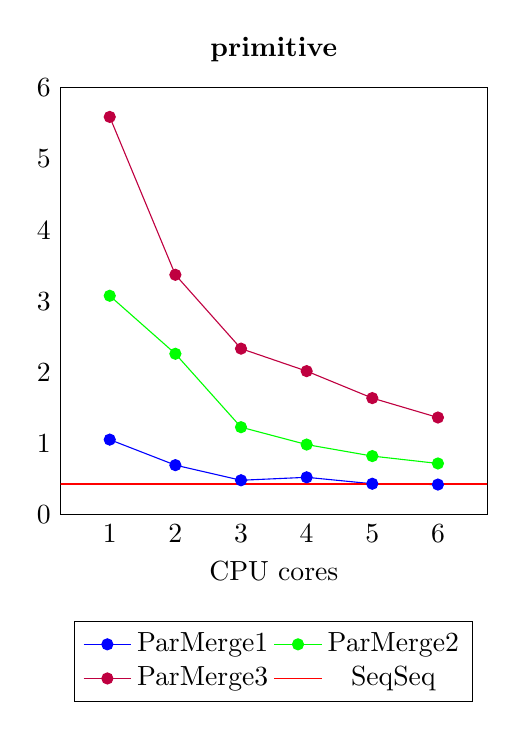
\begin{tikzpicture}
  \pgfplotsset{xtick style={draw=none}}
  \pgfplotsset{ytick style={draw=none}}
  \begin{axis}[
      width=7cm,
      height=7cm,
      enlargelimits=0.15,
      enlarge y limits=0,
      ymax=6,
      ymin=0,
      ytick distance=1,
      xtick=data,
      xlabel={CPU cores},
      xmin=1,
      xmax=6,
      xtick distance=1,
      title={\textbf{primitive}},
      legend style={
        at={(0.5,-0.25)},
        anchor=north,legend columns=2
      }
    ]
    \addplot[mark=*, blue] coordinates {
      (1,	1.05326)
      (2,	0.69427)
      (3,	0.48173)
      (4,	0.52334)
      (5,	0.43274)
      (6,	0.42144)
    };
    \addplot[mark=*, green] coordinates {
      (1,	3.07639)
      (2,	2.26061)
      (3,	1.22804)
      (4,	0.98374)
      (5,	0.82185)
      (6,	0.71797)
    };
    \addplot[mark=*, purple] coordinates {
      (1,	5.59171)
      (2,	3.37113)
      (3,	2.33293)
      (4,	2.01662)
      (5,	1.63729)
      (6,	1.36420)
    };
    \addplot[mark=none, red] coordinates {
      (0,0.429)
      (7,0.429)
    };
    \legend{ParMerge1, ParMerge2, ParMerge3, SeqSeq}
  \end{axis}
\end{tikzpicture}
~\hspace{-5pt}
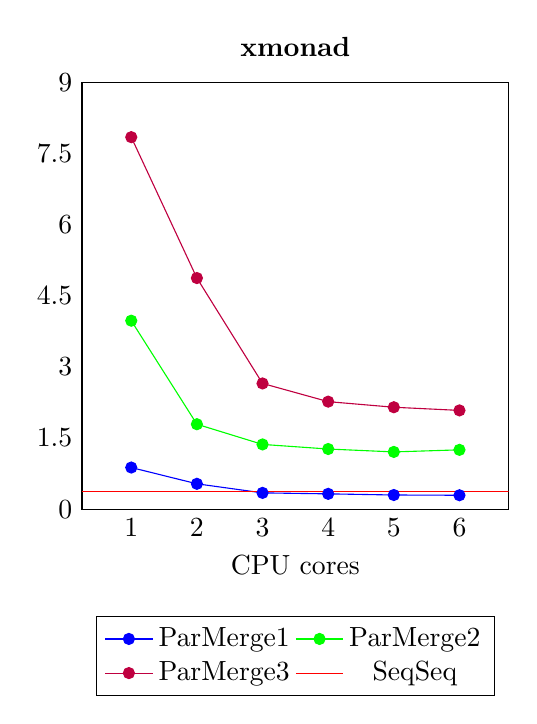
\begin{tikzpicture}
  \pgfplotsset{xtick style={draw=none}}
  \pgfplotsset{ytick style={draw=none}}
  \begin{axis}[
      width=7cm,
      height=7cm,
      enlargelimits=0.15,
      enlarge y limits=0,
      ymax=9,
      ymin=0,
      ytick distance=1.5,
      xtick=data,
      xlabel={CPU cores},
      xmin=1,
      xmax=6,
      xtick distance=1,
      title={\textbf{xmonad}},
      legend style={
        at={(0.5,-0.25)},
        anchor=north,legend columns=2
      }
    ]
    \addplot[mark=*, blue] coordinates {
      (1,	0.87770)
      (2,	0.53411)
      (3,	0.34285)
      (4,	0.32238)
      (5,	0.29815)
      (6,	0.29287)
    };
    \addplot[mark=*, green] coordinates {
      (1,	3.97514)
      (2,	1.79136)
      (3,	1.36511)
      (4,	1.26820)
      (5,	1.20695)
      (6,	1.25081)
    };
    \addplot[mark=*, purple] coordinates {
      (1,	7.84677)
      (2,	4.87466)
      (3,	2.65140)
      (4,	2.26753)
      (5,	2.14944)
      (6,	2.08265)
    };
    \addplot[mark=none, red] coordinates {
      (0,0.368)
      (7,0.368)
    };
    \legend{ParMerge1, ParMerge2, ParMerge3, SeqSeq}
  \end{axis}
\end{tikzpicture}
}

\subsection*{Parallel Projection}

\includegraphics[scale=0.3]{threadscope/ParProject1}

\includegraphics[scale=0.3]{threadscope/ParProject2}


% Parallel project
\resizebox{\textwidth}{!}{
\hspace{-50pt}
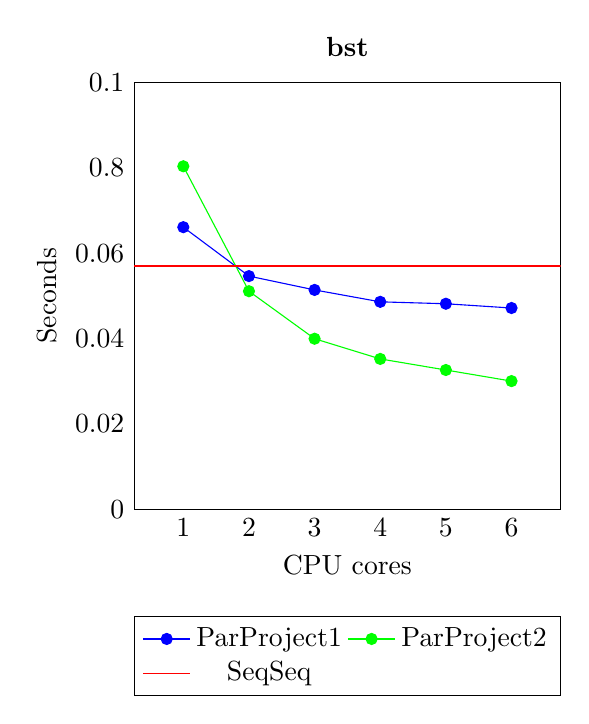
\begin{tikzpicture}
  \pgfplotsset{xtick style={draw=none}}
  \pgfplotsset{ytick style={draw=none}}
  \begin{axis}[
      width=7cm,
      height=7cm,
      enlargelimits=0.15,
      enlarge y limits=0,
      ymax=0.1,
      ymin=0,
      ytick distance=0.02,
      yticklabels={0,0,0.02,0.04,0.06,0.8,0.1},
      xtick=data,
      ylabel={Seconds},
      xlabel={CPU cores},
      xmin=1,
      xmax=6,
      xtick distance=1,
      title={\textbf{bst}},
      legend style={
        at={(0.5,-0.25)},
        anchor=north,legend columns=2
      }
    ]
    \addplot[mark=*, blue] coordinates {
      (1,	0.06609)
      (2,	0.05462)
      (3,	0.05138)
      (4,	0.04859)
      (5,	0.04814)
      (6,	0.04714)
    };
    \addplot[mark=*, green] coordinates {
      (1,	0.08036)
      (2,	0.05108)
      (3,	0.03994)
      (4,	0.03521)
      (5,	0.03261)
      (6,	0.03001)
    };
    \addplot[mark=none, red] coordinates {
      (0,0.0570)
      (7,0.0570)
    };
    \legend{ParProject1, ParProject2, SeqSeq}
  \end{axis}
\end{tikzpicture}
~\hspace{-5pt}
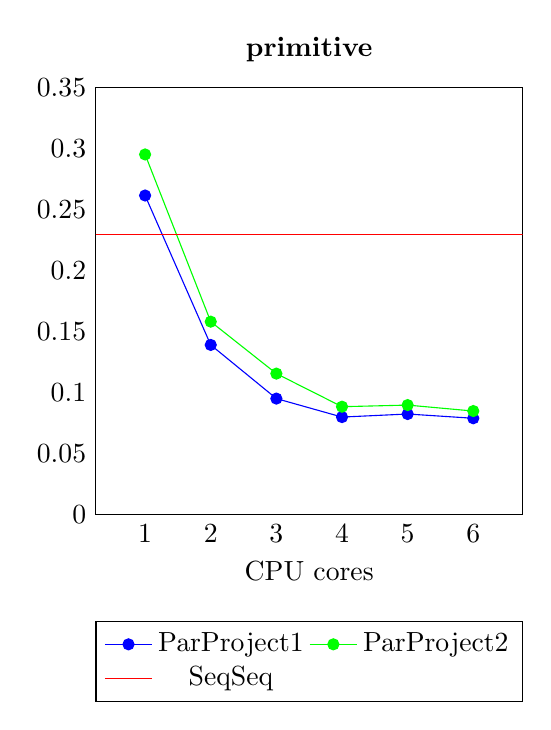
\begin{tikzpicture}
  \pgfplotsset{xtick style={draw=none}}
  \pgfplotsset{ytick style={draw=none}}
  \begin{axis}[
      width=7cm,
      height=7cm,
      enlargelimits=0.15,
      enlarge y limits=0,
      ymax=0.35,
      ymin=0,
      ytick distance=0.05,
      yticklabels={0,0,0.05,0.1,0.15,0.2,0.25,0.3,0.35},
      xtick=data,
      xlabel={CPU cores},
      xmin=1,
      xmax=6,
      xtick distance=1,
      title={\textbf{primitive}},
      legend style={
        at={(0.5,-0.25)},
        anchor=north,legend columns=2
      }
    ]
    \addplot[mark=*, blue] coordinates {
      (1,	0.26171)
      (2,	0.13912)
      (3,	0.09510)
      (4,	0.07994)
      (5,	0.08245)
      (6,	0.07896)
    };
    \addplot[mark=*, green] coordinates {
      (1,	0.29538)
      (2,	0.15821)
      (3,	0.11559)
      (4,	0.08845)
      (5,	0.08977)
      (6,	0.08489)
    };
    \addplot[mark=none, red] coordinates {
      (0,0.230)
      (7,0.230)
    };
    \legend{ParProject1, ParProject2, SeqSeq}
  \end{axis}
\end{tikzpicture}
~\hspace{-5pt}
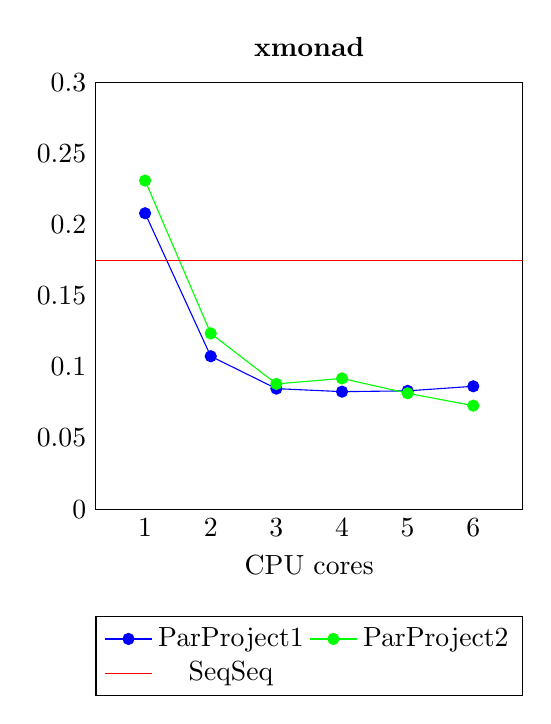
\begin{tikzpicture}
  \pgfplotsset{xtick style={draw=none}}
  \pgfplotsset{ytick style={draw=none}}
  \begin{axis}[
      width=7cm,
      height=7cm,
      enlargelimits=0.15,
      enlarge y limits=0,
      ymax=0.3,
      ymin=0,
      ytick distance=0.05,
      yticklabels={0,0,0.05,0.1,0.15,0.2,0.25,0.3},
      xtick=data,
      xlabel={CPU cores},
      xmin=1,
      xmax=6,
      xtick distance=1,
      title={\textbf{xmonad}},
      legend style={
        at={(0.5,-0.25)},
        anchor=north,legend columns=2
      }
    ]
    \addplot[mark=*, blue] coordinates {
      (1,	0.20805)
      (2,	0.10750)
      (3,	0.08473)
      (4,	0.08261)
      (5,	0.08317)
      (6,	0.08638)
    };
    \addplot[mark=*, green] coordinates {
      (1,	0.23102)
      (2,	0.12359)
      (3,	0.08807)
      (4,	0.09192)
      (5,	0.08147)
      (6,	0.07275)
    };
    \addplot[mark=none, red] coordinates {
      (0,0.175)
      (7,0.175)
    };
    \legend{ParProject1, ParProject2, SeqSeq}
  \end{axis}
\end{tikzpicture}
}

\subsection*{Parallel Coverage}

\includegraphics[scale=0.3]{threadscope/ParCoverage1}

\includegraphics[scale=0.3]{threadscope/ParCoverage2}

% Parallel coverage
\resizebox{\textwidth}{!}{
\hspace{-50pt}
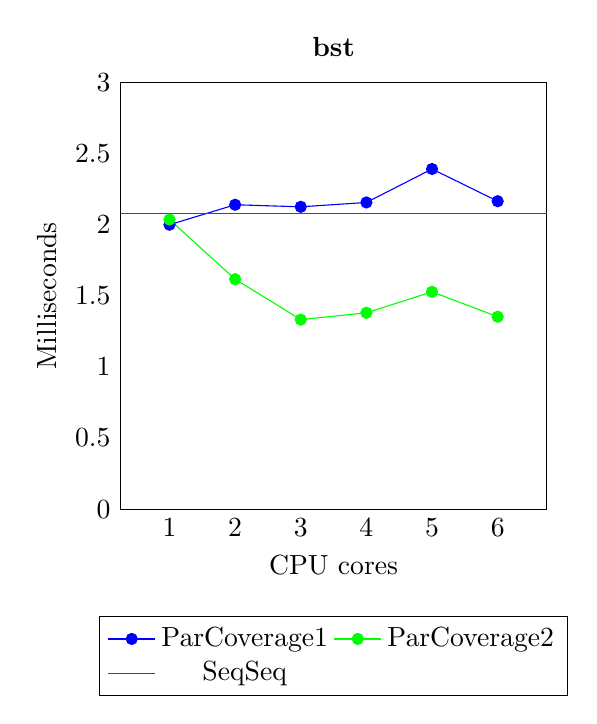
\begin{tikzpicture}
  \pgfplotsset{xtick style={draw=none}}
  \pgfplotsset{ytick style={draw=none}}
  \begin{axis}[
      width=7cm,
      height=7cm,
      enlargelimits=0.15,
      enlarge y limits=0,
      ymax=3,
      ymin=0,
      ytick distance=0.5,
      yticklabels={0,0,0.5,1,1.5,2,2.5,3},
      xtick=data,
      ylabel={Milliseconds},
      xlabel={CPU cores},
      xmin=1,
      xmax=6,
      xtick distance=1,
      title={\textbf{bst}},
      legend style={
        at={(0.5,-0.25)},
        anchor=north,legend columns=2
      }
    ]
    \addplot[mark=*, blue] coordinates {
      (1,	1.999798457)
      (2,	2.140306418)
      (3,	2.125807102)
      (4,	2.156469454)
      (5,	2.391723436)
      (6,	2.16521249)
    };
    \addplot[mark=*, green] coordinates {
      (1,	2.036091602)
      (2,	1.616879328)
      (3,	1.332552591)
      (4,	1.380659664)
      (5,	1.52799736)
      (6,	1.352924105)
    };
    \addplot[mark=none, red] coordinates {
      (0,2.076)
      (7,2.076)
    };
    \legend{ParCoverage1, ParCoverage2, SeqSeq}
  \end{axis}
\end{tikzpicture}
~\hspace{-5pt}
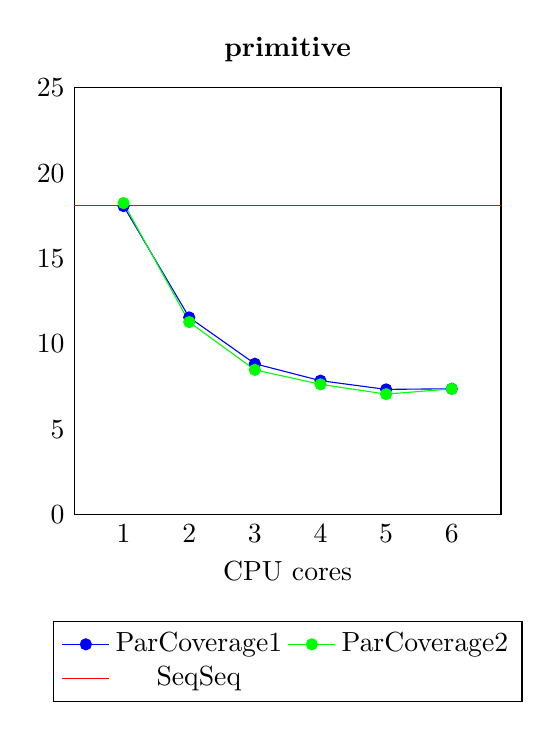
\begin{tikzpicture}
  \pgfplotsset{xtick style={draw=none}}
  \pgfplotsset{ytick style={draw=none}}
  \begin{axis}[
      width=7cm,
      height=7cm,
      enlargelimits=0.15,
      enlarge y limits=0,
      ymax=25,
      ymin=0,
      ytick distance=5,
      xtick=data,
      xlabel={CPU cores},
      xmin=1,
      xmax=6,
      xtick distance=1,
      title={\textbf{primitive}},
      legend style={
        at={(0.5,-0.25)},
        anchor=north,legend columns=2
      }
    ]
    \addplot[mark=*, blue] coordinates {
      (1,	18.07241404)
      (2,	11.54932487)
      (3,	8.835522228)
      (4,	7.843209439)
      (5,	7.331879587)
      (6,	7.369470515)
    };
    \addplot[mark=*, green] coordinates {
      (1,	18.24999386)
      (2,	11.27700625)
      (3,	8.477055719)
      (4,	7.628884595)
      (5,	7.054208489)
      (6,	7.363956561)
    };
    \addplot[mark=none, red] coordinates {
      (0,18.09)
      (7,18.09)
    };
    \legend{ParCoverage1, ParCoverage2, SeqSeq}
  \end{axis}
\end{tikzpicture}
~\hspace{-5pt}
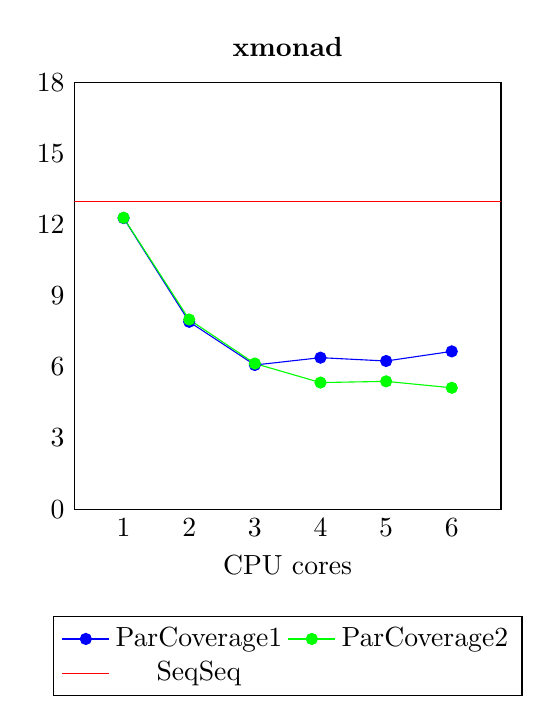
\begin{tikzpicture}
  \pgfplotsset{xtick style={draw=none}}
  \pgfplotsset{ytick style={draw=none}}
  \begin{axis}[
      width=7cm,
      height=7cm,
      enlargelimits=0.15,
      enlarge y limits=0,
      ymax=18,
      ymin=0,
      ytick distance=3,
      xtick=data,
      xlabel={CPU cores},
      xmin=1,
      xmax=6,
      xtick distance=1,
      title={\textbf{xmonad}},
      legend style={
        at={(0.5,-0.25)},
        anchor=north,legend columns=2
      }
    ]
    \addplot[mark=*, blue] coordinates {
      (1,	12.27925829)
      (2,	7.903431115)
      (3,	6.080712386)
      (4,	6.390404331)
      (5,	6.249881708)
      (6,	6.65609943)
    };
    \addplot[mark=*, green] coordinates {
      (1,	12.29389248)
      (2,	7.998992073)
      (3,	6.142958556)
      (4,	5.339186735)
      (5,	5.391108887)
      (6,	5.120059685)
    };
    \addplot[mark=none, red] coordinates {
      (0,12.98)
      (7,12.98)
    };
    \legend{ParCoverage1, ParCoverage2, SeqSeq}
  \end{axis}
\end{tikzpicture}
}

%%%%%%%%%%%%%%%%%%%%%%%%%%%%%%%%%%%%%%%%
% Bibliography

\begin{thebibliography}{}

  \bibitem{baker} Baker, N. 1966, in Stellar Evolution, ed.\ R. F. Stein \& A.
    G. W. Cameron (Plenum, New York) 333

   \bibitem{zheng} Zheng, W., Davidsen, A. F., Tytler, D. \& Kriss, G. A. 1997,
     preprint

\end{thebibliography}

\end{document}
